% !TeX root = ../main.tex

\chapter{ASSD目标检测器}

\section{ASSD简介}

ASSD\cite{ASSD}是一阶段基于候选框的注意力目标检测网络,其是以SSD\cite{SSD}为原型并进行改进的。
SSD虽然能够对多尺度特征映射进行检测,还能够有效地处理各种类别大小,但是,其小尺度金字塔结构层缺乏语义信息,因此小目标识别的效果不好。解决这一问题的一种方法是建立更多的卷积层,对涉及到的小目标特征进行进一步的细化,或者将语义较多的从大尺度层传入到小尺度层。考虑到速度是一阶段目标探测器的主要优势,故需要用以较小的额外计算成本提高SSD的精度。为了达到这样的目的,ASSD方法构建了一个小型注意单元网络,将SSD输出的特征图放入运算,以提高检测结果的准确性。ASSD将注意力单元放在特征映射和预测模块之间。ASSD选择SSD作为一级探测器,它在简单性、速度和准确性之间提供了最佳的权衡,它保留了SSD的原始结构,并且在小尺度层引入了融合机制来加入语义信息。这种设计保留了原始SSD的优点,同时更有效地学习对象特性。在PASCAL VOC和COCO等数据集上,ASSD在精度和效率方面的表现的比之前所有的一阶段目标检测器更好。鉴于ASSD强大的性能,我们决定在实验中选取ASSD作为检测器。



\section{网络整体结构}

ASSD的整体结构如图\ref{ASSDStructure}所示:

\begin{figure}
	\center
	{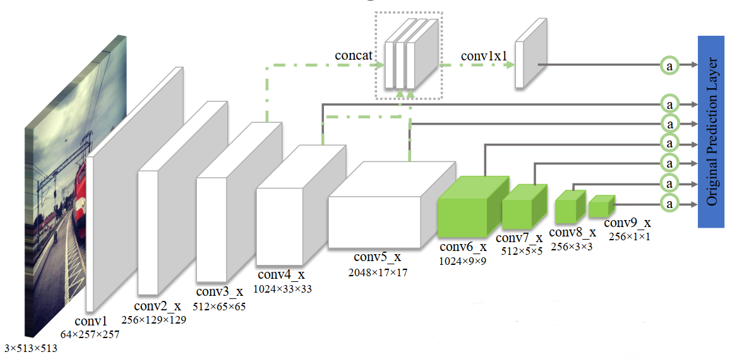
\includegraphics[width=16cm,height=8cm]{ASSDStructure.png}}
	\caption{ASSD整体结构示意图}
	\label{ASSDStructure}
\end{figure}


ASSD总共进行九层卷积操作。其中第 、四、五次的卷积通过语义融合输出特征图,四到九的卷积依次输出特征图,然后将这七份特征图都放入注意力单元进行运算,最后进行回归分类,得出预测结果。

\section{候选框}
%输入网络之前需要对图片进行处理:

%1.填充至宽高相等。

%2.分辨率放缩至$513\times 513$。

如图\ref{AnchorDemo}所示,首先将输入图片进行填充至宽高相等,然后resize至513×513分辨率作为输入,之后不同的金字塔模块对图像分割处理的方式不同。

\begin{figure}
	\center
	{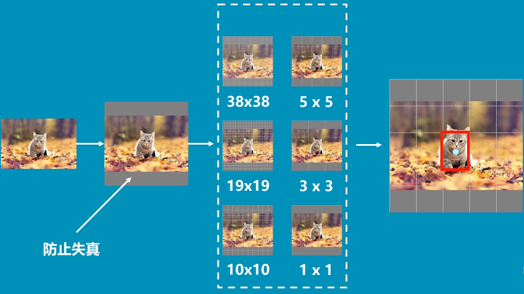
\includegraphics[width=10cm,height=6cm]{AnchorDemo.png}}
	\caption{不同层对图片的划分}
	\label{AnchorDemo}
\end{figure}


对于小目标的检测集中于宽高划分小的层中(如$38\times 38$,$19\times 19$),大目标的检测位于宽高划分大的金字塔模块中(如$1\times 1$,$3\times $3)。

\begin{figure}
	\center
	{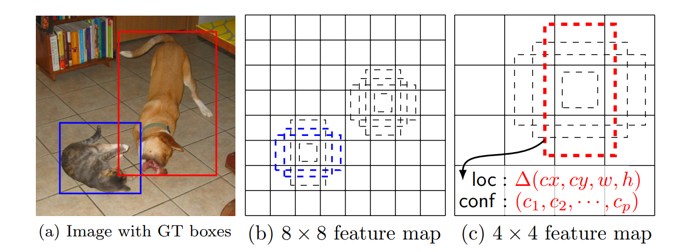
\includegraphics[width=15cm,height=5cm]{SSDAnchor.png}}
	\caption{SSD中的Anchor机制}
	\label{SSDAnchor}
\end{figure}

如图\ref{SSDAnchor}所示,在固定划分的情况下,对于特征图上的一个具体正方形会生成若干种不同尺寸、宽高比的候选框,网络会对所有的候选框进行检测,然后进行分类回归得到置信度,之后与Ground Truth比较得出loss反向传播更新权值。

\begin{figure}
	\center
	{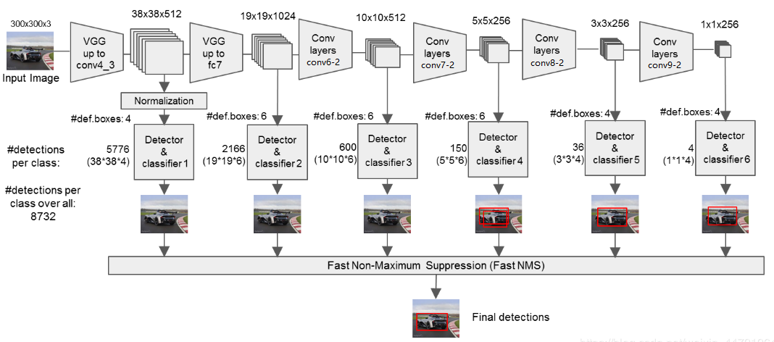
\includegraphics[width=16cm,height=7cm]{SSDDetect.png}}
	\caption{每层的Anchor}
	\label{SSDDetect}
\end{figure}

如图\ref{SSDDetect}所示,以第一层为例:该层将输入图片划分成$38\times 38$的方格,每一个方格都会生成4个Anchor,于是该层总共有$38\times 38\times 4=5776$个Anchor

ASSD采用与SSD相同的Anchor Box生成方法。

具体来说,使用长宽比$a_{r}={1,2,1/_2}$作为特征映射conv3,8,9上的Anchor Box,使用$a_{r}={1,2,1/_2,3,1/_3}$作为特征映射conv4-7上的Anchor Box。每个Box都有一个最小尺度$s_{min}$和一个最大尺度$s_{max}$。
Anchor Box的标准化宽度和高度按$w=s\sqrt(a_{r} )$和$h=s/\sqrt{a_{r}}$计算,其中
\begin{equation}
s=\left\{\begin{matrix}
\sqrt{s_{min}\times s_{max}},a_{r}=1\\ 
s_{min},\,otherwise
\end{matrix}\right.
\end{equation}

%$s=\sqrt{s_{min}\times s_{max}},(a_{r}=1)$ ,否则$s=s_{min}$。

其使用了7个不同尺寸的特征图来进行预测,分别是($65\times 65$),($33\times 33$),($17\times 17$),($9\times 9$),($5\times 5$),($3\times 3$),($1\times 1$)。第一、六、七层对每个位置使用4种候选框进行预测,其余层使用6种。

故对于七层金字塔结构的ASSD,对于每张图片其总共检测$(65×65)×4+(33×33)×6+(17×17)×6+(9×9)×6+(5×5)×6+(3×3)×4+(1×1)×4=25844$个候选框。


\section{融合机制}
ASSD受FSSD的启发,它将layer4和layer5的提取到的特征图(即上下文信息)融合到layer3中,以增添其语义。实验中,单独的融合操作并不能显著提高检测精度。相反,从实验结果来看,它甚至降低了精度一点与更多的计算成本。这主要是因为这三层结构具有着不同的感受野和不同的提取特征的能力;此外,级联和1$\times$1的卷子操作可能会抵消三层之间的相对重要性,并抑制了原始layer3层中的关键特征。实验表明,在融合后放置注意力单元时,效果会有明显的改善。深层语义的引入帮助了注意单元,让它可以发现存在于原始layer3层中的有用信息。如果只使用注意单元时,其效果与融合和注意机制模型相比性能较差。如图\ref{FusionAtt}所示,这说明特征融合机制和注意力单元是相辅相成的,也就是说要同时使用这两个机制对模型进行训练。

\begin{figure}
	\center
	{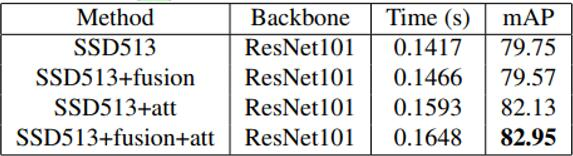
\includegraphics[width=7.5cm,height=2cm]{FusionAtt.jpg}}
	\caption{特征融合与注意力机制的表现}
	\label{FusionAtt}
\end{figure}

语义融合的过程可以表示为:
\begin{equation}
	x^3=W^3Concat{x^3,x^4,x^5}+b^3
\end{equation}
其中$x^s\in R^{c^s\times N^s}$是$s$层的特征图,$W^3\in R^{C^3\times C'}$,$b^3\in R^{C^3}$。

$Concat$操作通过双线性插值对第四层和第五层进行上采样,以使其大小与第三层的大小对齐,从而能够输出三层间的综合特征,如图\ref{Fusion}所示。

\begin{figure}
	\center
	{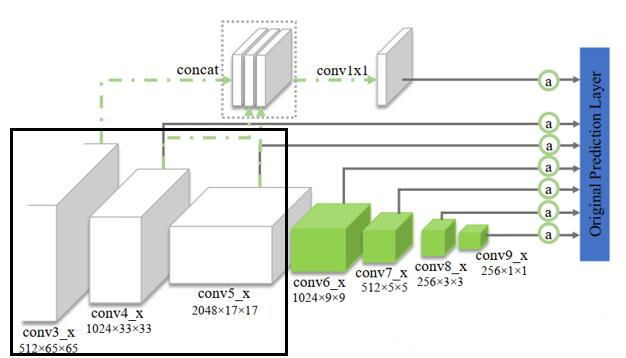
\includegraphics[width=12.52cm,height=7.16cm]{Fusion.jpg}}
	\caption{融合}
	\label{Fusion}
\end{figure}

\section{注意力单元}

\begin{figure}
	\center
	{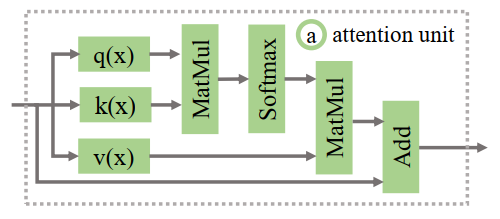
\includegraphics[width=10cm,height=4cm]{AttUnit.png}}
	\caption{注意力单元示意图}
	\label{AttUnit}
\end{figure}

注意力单元如图\ref{AttUnit}所示,其具体计算方式如下:

假设$x^s\in R^{C^s\times N^s}$是$s$层的特征图,进行如下操作:

\begin{equation}
	q(x^s)={W_q^{s}}^Tx^s\in R^{C'\times N^S}
\end{equation}

\begin{equation}
	k(x^s)={W_k^{s}}^Tx^s\in R^{C'\times N^S}
\end{equation}

\begin{equation}
	v(x^s)={W_v^{s}}^Tx^s\in R^{C^s\times N^S}
\end{equation}


其中
\begin{equation}
	W_q^{s},W_k^{s}\in R^{C^s\times C'} , 
	W_v^{s}\in R^{C^s\times C^s}
\end{equation}

设$a^s$为注意力得分矩阵,其产生如下:

\begin{equation}
	a^s={q(x^s)}^Tk(x^s)\in R^{N^s\times N^s}
\end{equation}


将$a^s$每一行通过$softmax$操作规范化:
\begin{equation}
	\bar a^s_{ij}=\frac{exp(a^s_{ij})}{\Sigma^{N^S}_jexp(a^s_{ij})},i,j=1,2,\cdots,N^S
\end{equation}


其中$\bar a^s_{i}$表示查询特征图的第$i$个位置时的像素关系,称之为“注意力图”。将输入特性$x^s$转换为$q$和$k$的原因是为了减小矩阵运算的开销、降低计算成本。$q(x^s)$和$k(x^s)$的矩阵计算特征相似度,并创建一个$N\times N$注意力图,以便显示特征之间的关系。
接下来,我们应用$v(x^s)$和注意图$a^s$之间的乘法操作。使用这种运算,我们通过计算一个更新后的的特征图,作为每个位置上的单个特征的加权和。最后,我们将之前的矩阵乘法结果添加回输入特征映射$x^s$中:

\begin{equation}
	x^{s'}=x^s+{(\bar a^s v(x^s)^T)}^T
\end{equation}

注意力图$\bar a^s$将特征图在所有位置的大范围关系联系起来,因此学习了特征图的全局上下文。它突出了特征图的相关部分,并以细化的信息指导检测。

\section{损失函数}
训练过程中的$loss$为置信度的损失函数$loss\_conf$与预测边框的损失函数$loss\_locs$之和:

\begin{equation}
	loss = loss_l + loss_c
\end{equation}

其中,$loss\_conf$为Pytorch中计算交叉熵的$F.cross\_entropy$,计算方式如下:
\begin{equation}
	loss(x,class)=-log(\frac{exp(x[class])}{\Sigma_jexp(x[j])})
\end{equation}

$loss\_locs$使用$Smooth L1$作为损失函数,计算方法如下:
\begin{equation}
	Smooth L1(x)=\left\{\begin{matrix}
	0.5x^2,\,\,\,\,\,\,\,\,if |x|<1\\ 
	|x|-0.5,\,otherwise
	\end{matrix}\right.
\end{equation}

其中,$s=f(x_i)-y_i$为真实值和预测值的差值。
